\documentclass[]{book}
\usepackage{lmodern}
\usepackage{amssymb,amsmath}
\usepackage{ifxetex,ifluatex}
\usepackage{fixltx2e} % provides \textsubscript
\ifnum 0\ifxetex 1\fi\ifluatex 1\fi=0 % if pdftex
  \usepackage[T1]{fontenc}
  \usepackage[utf8]{inputenc}
\else % if luatex or xelatex
  \ifxetex
    \usepackage{mathspec}
  \else
    \usepackage{fontspec}
  \fi
  \defaultfontfeatures{Ligatures=TeX,Scale=MatchLowercase}
\fi
% use upquote if available, for straight quotes in verbatim environments
\IfFileExists{upquote.sty}{\usepackage{upquote}}{}
% use microtype if available
\IfFileExists{microtype.sty}{%
\usepackage{microtype}
\UseMicrotypeSet[protrusion]{basicmath} % disable protrusion for tt fonts
}{}
\usepackage[margin=1in]{geometry}
\usepackage{hyperref}
\hypersetup{unicode=true,
            pdftitle={Homework2},
            pdfauthor={Jieying Jiao},
            pdfborder={0 0 0},
            breaklinks=true}
\urlstyle{same}  % don't use monospace font for urls
\usepackage{natbib}
\bibliographystyle{apalike}
\usepackage{color}
\usepackage{fancyvrb}
\newcommand{\VerbBar}{|}
\newcommand{\VERB}{\Verb[commandchars=\\\{\}]}
\DefineVerbatimEnvironment{Highlighting}{Verbatim}{commandchars=\\\{\}}
% Add ',fontsize=\small' for more characters per line
\usepackage{framed}
\definecolor{shadecolor}{RGB}{248,248,248}
\newenvironment{Shaded}{\begin{snugshade}}{\end{snugshade}}
\newcommand{\AlertTok}[1]{\textcolor[rgb]{0.94,0.16,0.16}{#1}}
\newcommand{\AnnotationTok}[1]{\textcolor[rgb]{0.56,0.35,0.01}{\textbf{\textit{#1}}}}
\newcommand{\AttributeTok}[1]{\textcolor[rgb]{0.77,0.63,0.00}{#1}}
\newcommand{\BaseNTok}[1]{\textcolor[rgb]{0.00,0.00,0.81}{#1}}
\newcommand{\BuiltInTok}[1]{#1}
\newcommand{\CharTok}[1]{\textcolor[rgb]{0.31,0.60,0.02}{#1}}
\newcommand{\CommentTok}[1]{\textcolor[rgb]{0.56,0.35,0.01}{\textit{#1}}}
\newcommand{\CommentVarTok}[1]{\textcolor[rgb]{0.56,0.35,0.01}{\textbf{\textit{#1}}}}
\newcommand{\ConstantTok}[1]{\textcolor[rgb]{0.00,0.00,0.00}{#1}}
\newcommand{\ControlFlowTok}[1]{\textcolor[rgb]{0.13,0.29,0.53}{\textbf{#1}}}
\newcommand{\DataTypeTok}[1]{\textcolor[rgb]{0.13,0.29,0.53}{#1}}
\newcommand{\DecValTok}[1]{\textcolor[rgb]{0.00,0.00,0.81}{#1}}
\newcommand{\DocumentationTok}[1]{\textcolor[rgb]{0.56,0.35,0.01}{\textbf{\textit{#1}}}}
\newcommand{\ErrorTok}[1]{\textcolor[rgb]{0.64,0.00,0.00}{\textbf{#1}}}
\newcommand{\ExtensionTok}[1]{#1}
\newcommand{\FloatTok}[1]{\textcolor[rgb]{0.00,0.00,0.81}{#1}}
\newcommand{\FunctionTok}[1]{\textcolor[rgb]{0.00,0.00,0.00}{#1}}
\newcommand{\ImportTok}[1]{#1}
\newcommand{\InformationTok}[1]{\textcolor[rgb]{0.56,0.35,0.01}{\textbf{\textit{#1}}}}
\newcommand{\KeywordTok}[1]{\textcolor[rgb]{0.13,0.29,0.53}{\textbf{#1}}}
\newcommand{\NormalTok}[1]{#1}
\newcommand{\OperatorTok}[1]{\textcolor[rgb]{0.81,0.36,0.00}{\textbf{#1}}}
\newcommand{\OtherTok}[1]{\textcolor[rgb]{0.56,0.35,0.01}{#1}}
\newcommand{\PreprocessorTok}[1]{\textcolor[rgb]{0.56,0.35,0.01}{\textit{#1}}}
\newcommand{\RegionMarkerTok}[1]{#1}
\newcommand{\SpecialCharTok}[1]{\textcolor[rgb]{0.00,0.00,0.00}{#1}}
\newcommand{\SpecialStringTok}[1]{\textcolor[rgb]{0.31,0.60,0.02}{#1}}
\newcommand{\StringTok}[1]{\textcolor[rgb]{0.31,0.60,0.02}{#1}}
\newcommand{\VariableTok}[1]{\textcolor[rgb]{0.00,0.00,0.00}{#1}}
\newcommand{\VerbatimStringTok}[1]{\textcolor[rgb]{0.31,0.60,0.02}{#1}}
\newcommand{\WarningTok}[1]{\textcolor[rgb]{0.56,0.35,0.01}{\textbf{\textit{#1}}}}
\usepackage{longtable,booktabs}
\usepackage{graphicx,grffile}
\makeatletter
\def\maxwidth{\ifdim\Gin@nat@width>\linewidth\linewidth\else\Gin@nat@width\fi}
\def\maxheight{\ifdim\Gin@nat@height>\textheight\textheight\else\Gin@nat@height\fi}
\makeatother
% Scale images if necessary, so that they will not overflow the page
% margins by default, and it is still possible to overwrite the defaults
% using explicit options in \includegraphics[width, height, ...]{}
\setkeys{Gin}{width=\maxwidth,height=\maxheight,keepaspectratio}
\IfFileExists{parskip.sty}{%
\usepackage{parskip}
}{% else
\setlength{\parindent}{0pt}
\setlength{\parskip}{6pt plus 2pt minus 1pt}
}
\setlength{\emergencystretch}{3em}  % prevent overfull lines
\providecommand{\tightlist}{%
  \setlength{\itemsep}{0pt}\setlength{\parskip}{0pt}}
\setcounter{secnumdepth}{5}
% Redefines (sub)paragraphs to behave more like sections
\ifx\paragraph\undefined\else
\let\oldparagraph\paragraph
\renewcommand{\paragraph}[1]{\oldparagraph{#1}\mbox{}}
\fi
\ifx\subparagraph\undefined\else
\let\oldsubparagraph\subparagraph
\renewcommand{\subparagraph}[1]{\oldsubparagraph{#1}\mbox{}}
\fi

%%% Use protect on footnotes to avoid problems with footnotes in titles
\let\rmarkdownfootnote\footnote%
\def\footnote{\protect\rmarkdownfootnote}

%%% Change title format to be more compact
\usepackage{titling}

% Create subtitle command for use in maketitle
\newcommand{\subtitle}[1]{
  \posttitle{
    \begin{center}\large#1\end{center}
    }
}

\setlength{\droptitle}{-2em}

  \title{Homework2}
    \pretitle{\vspace{\droptitle}\centering\huge}
  \posttitle{\par}
    \author{Jieying Jiao}
    \preauthor{\centering\large\emph}
  \postauthor{\par}
      \predate{\centering\large\emph}
  \postdate{\par}
    \date{2018-09-12}

\usepackage{booktabs}

\begin{document}
\maketitle

{
\setcounter{tocdepth}{1}
\tableofcontents
}
\hypertarget{exercise-1.2}{%
\chapter{Exercise 1.2}\label{exercise-1.2}}

\hypertarget{use-monte-carlo-to-estimate-phit}{%
\section{\texorpdfstring{Use Monte Carlo to estimate
\(\Phi(t)\)}{Use Monte Carlo to estimate \textbackslash{}Phi(t)}}\label{use-monte-carlo-to-estimate-phit}}

The Monte Carlo methods gives:

\[\hat{\Phi}(t) = \frac{1}{n}\sum_{i = 1}^nI(X_i\leqslant t)\] where
\(X_i\) are random normal sample drawn from \(N(0, 1)\).

\begin{Shaded}
\begin{Highlighting}[]
\KeywordTok{library}\NormalTok{(xtable)}
\NormalTok{phi.MC <-}\StringTok{ }\ControlFlowTok{function}\NormalTok{(n, t) \{}
\NormalTok{  phi.hat <-}\StringTok{ }\KeywordTok{matrix}\NormalTok{(}\DecValTok{0}\NormalTok{, }\DataTypeTok{nrow =} \KeywordTok{length}\NormalTok{(n), }\DataTypeTok{ncol =} \KeywordTok{length}\NormalTok{(t))}
  \ControlFlowTok{for}\NormalTok{ (i }\ControlFlowTok{in} \DecValTok{1}\OperatorTok{:}\KeywordTok{length}\NormalTok{(n)) \{}
    \ControlFlowTok{for}\NormalTok{ (j }\ControlFlowTok{in} \DecValTok{1}\OperatorTok{:}\KeywordTok{length}\NormalTok{(t)) \{}
\NormalTok{      X <-}\StringTok{ }\KeywordTok{rnorm}\NormalTok{(n[i], }\DecValTok{0}\NormalTok{, }\DecValTok{1}\NormalTok{)}
\NormalTok{      phi.hat[i, j] <-}\StringTok{ }\KeywordTok{mean}\NormalTok{(}\KeywordTok{as.numeric}\NormalTok{(X }\OperatorTok{<=}\StringTok{ }\NormalTok{t[j]))}
\NormalTok{    \}}
\NormalTok{  \}}
\NormalTok{truth <-}\StringTok{ }\KeywordTok{pnorm}\NormalTok{(t)}
\NormalTok{phi.hat <-}\StringTok{ }\KeywordTok{rbind}\NormalTok{(phi.hat, truth)}
\NormalTok{\}}
\NormalTok{n <-}\StringTok{ }\KeywordTok{c}\NormalTok{(}\DecValTok{10}\OperatorTok{^}\DecValTok{2}\NormalTok{, }\DecValTok{10}\OperatorTok{^}\DecValTok{3}\NormalTok{, }\DecValTok{10}\OperatorTok{^}\DecValTok{4}\NormalTok{)}
\NormalTok{t <-}\StringTok{ }\KeywordTok{c}\NormalTok{(}\FloatTok{0.0}\NormalTok{, }\FloatTok{0.67}\NormalTok{, }\FloatTok{0.84}\NormalTok{, }\FloatTok{1.28}\NormalTok{, }\FloatTok{1.65}\NormalTok{, }\FloatTok{2.32}\NormalTok{, }\FloatTok{2.58}\NormalTok{, }\FloatTok{3.09}\NormalTok{, }\FloatTok{3.72}\NormalTok{)}
\KeywordTok{set.seed}\NormalTok{(}\DecValTok{1}\NormalTok{)}
\NormalTok{phi.hat <-}\StringTok{ }\KeywordTok{phi.MC}\NormalTok{(n, t)}
\KeywordTok{rownames}\NormalTok{(phi.hat) <-}\StringTok{ }\KeywordTok{c}\NormalTok{(}\KeywordTok{paste0}\NormalTok{(}\StringTok{"n = 10e"}\NormalTok{, }\DecValTok{2}\OperatorTok{:}\DecValTok{4}\NormalTok{), }\StringTok{"truth"}\NormalTok{)}
\KeywordTok{colnames}\NormalTok{(phi.hat) <-}\StringTok{ }\KeywordTok{paste0}\NormalTok{(}\StringTok{"t = "}\NormalTok{, t)}
\NormalTok{t.MC <-}\StringTok{ }\KeywordTok{xtable}\NormalTok{(phi.hat, }\DataTypeTok{digits =} \DecValTok{4}\NormalTok{, }\DataTypeTok{caption =} \StringTok{"Monte Carlo estimation"}\NormalTok{, }
               \DataTypeTok{label =} \StringTok{"MC result"}\NormalTok{)}
\end{Highlighting}
\end{Shaded}

The estimation results are shown in Table \ref{MC result}.

\begin{table}[ht]
\centering
\begin{tabular}{rrrrrrrrrr}
  \hline
 & t = 0 & t = 0.67 & t = 0.84 & t = 1.28 & t = 1.65 & t = 2.32 & t = 2.58 & t = 3.09 & t = 3.72 \\ 
  \hline
n = 10e2 & 0.4600 & 0.7700 & 0.7800 & 0.8700 & 0.9200 & 1.0000 & 0.9900 & 1.0000 & 1.0000 \\ 
  n = 10e3 & 0.5110 & 0.7370 & 0.7710 & 0.9080 & 0.9500 & 0.9860 & 0.9990 & 0.9980 & 1.0000 \\ 
  n = 10e4 & 0.5061 & 0.7467 & 0.8021 & 0.8981 & 0.9527 & 0.9913 & 0.9947 & 0.9985 & 0.9998 \\ 
  truth & 0.5000 & 0.7486 & 0.7995 & 0.8997 & 0.9505 & 0.9898 & 0.9951 & 0.9990 & 0.9999 \\ 
   \hline
\end{tabular}
\caption{Monte Carlo estimation} 
\label{MC result}
\end{table}

\hypertarget{boxplots-of-bias}{%
\section{Boxplots of bias}\label{boxplots-of-bias}}

Repeat the above expriment 100 times and plot bias of Monte Carlo
methods at every time point \(t\) using boxplots.

\begin{Shaded}
\begin{Highlighting}[]
\KeywordTok{library}\NormalTok{(ggplot2)}
\NormalTok{nsim <-}\StringTok{ }\DecValTok{100}
\NormalTok{bias <-}\StringTok{ }\KeywordTok{data.frame}\NormalTok{(}\DataTypeTok{bias =} \KeywordTok{rep}\NormalTok{(}\DecValTok{0}\NormalTok{, nsim }\OperatorTok{*}\StringTok{ }\KeywordTok{length}\NormalTok{(t) }\OperatorTok{*}\StringTok{ }\KeywordTok{length}\NormalTok{(n)), }
                   \DataTypeTok{t =} \KeywordTok{rep}\NormalTok{(t, }\KeywordTok{length}\NormalTok{(n) }\OperatorTok{*}\StringTok{ }\NormalTok{nsim), }
                   \DataTypeTok{n =} \KeywordTok{rep}\NormalTok{(}\KeywordTok{rep}\NormalTok{(n, }\DataTypeTok{each =} \KeywordTok{length}\NormalTok{(t)), nsim))}
\ControlFlowTok{for}\NormalTok{ (i }\ControlFlowTok{in} \DecValTok{1}\OperatorTok{:}\NormalTok{nsim) \{}
\NormalTok{  phi.hat <-}\StringTok{ }\KeywordTok{phi.MC}\NormalTok{(n, t)}
\NormalTok{  bias}\OperatorTok{$}\NormalTok{bias[((i}\DecValTok{-1}\NormalTok{)}\OperatorTok{*}\KeywordTok{length}\NormalTok{(t)}\OperatorTok{*}\KeywordTok{length}\NormalTok{(n)}\OperatorTok{+}\DecValTok{1}\NormalTok{)}\OperatorTok{:}\NormalTok{(i}\OperatorTok{*}\KeywordTok{length}\NormalTok{(t)}\OperatorTok{*}\KeywordTok{length}\NormalTok{(n))] <-}\StringTok{ }
\StringTok{    }\KeywordTok{as.vector}\NormalTok{(}\KeywordTok{t}\NormalTok{(phi.hat[}\DecValTok{1}\OperatorTok{:}\KeywordTok{length}\NormalTok{(n), ]) }\OperatorTok{-}\StringTok{ }\NormalTok{phi.hat[}\KeywordTok{length}\NormalTok{(n) }\OperatorTok{+}\StringTok{ }\DecValTok{1}\NormalTok{, ])}
\NormalTok{\}}
\NormalTok{bias}\OperatorTok{$}\NormalTok{t <-}\StringTok{ }\KeywordTok{as.factor}\NormalTok{(bias}\OperatorTok{$}\NormalTok{t)}
\KeywordTok{ggplot}\NormalTok{(}\DataTypeTok{data =}\NormalTok{ bias, }\KeywordTok{aes}\NormalTok{(}\DataTypeTok{x =}\NormalTok{ t, }\DataTypeTok{y =}\NormalTok{ bias)) }\OperatorTok{+}\StringTok{ }
\StringTok{  }\KeywordTok{geom_boxplot}\NormalTok{(}\DataTypeTok{outlier.colour=}\StringTok{"red"}\NormalTok{, }\DataTypeTok{outlier.shape=}\DecValTok{8}\NormalTok{, }\DataTypeTok{outlier.size=}\DecValTok{4}\NormalTok{) }\OperatorTok{+}\StringTok{ }
\StringTok{  }\KeywordTok{facet_wrap}\NormalTok{( }\OperatorTok{~}\StringTok{ }\NormalTok{n) }\OperatorTok{+}\StringTok{ }\KeywordTok{theme}\NormalTok{(}\DataTypeTok{text =} \KeywordTok{element_text}\NormalTok{(}\DataTypeTok{size =} \DecValTok{10}\NormalTok{))}
\end{Highlighting}
\end{Shaded}

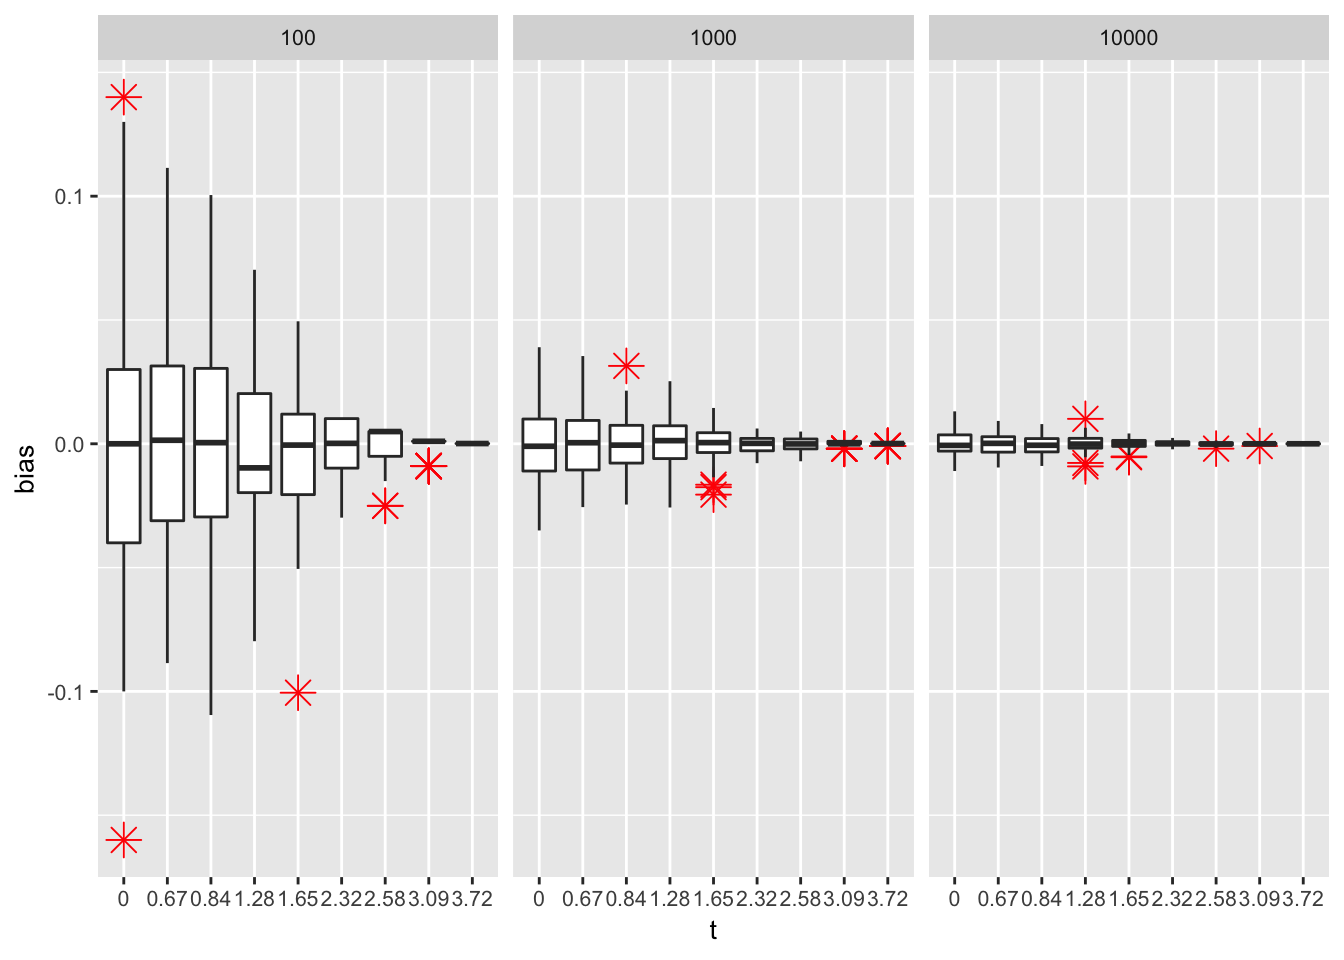
\includegraphics{Homework2-JieyingJiao_files/figure-latex/Homework2_2-1.pdf}

\hypertarget{exercise-1.3}{%
\chapter{Exercise 1.3}\label{exercise-1.3}}

\begin{Shaded}
\begin{Highlighting}[]
\NormalTok{.Machine}\OperatorTok{$}\NormalTok{double.xmax }
\end{Highlighting}
\end{Shaded}

\begin{verbatim}
## [1] 1.797693e+308
\end{verbatim}

\begin{Shaded}
\begin{Highlighting}[]
\NormalTok{.Machine}\OperatorTok{$}\NormalTok{double.xmin}
\end{Highlighting}
\end{Shaded}

\begin{verbatim}
## [1] 2.225074e-308
\end{verbatim}

\begin{Shaded}
\begin{Highlighting}[]
\NormalTok{.Machine}\OperatorTok{$}\NormalTok{double.eps}
\end{Highlighting}
\end{Shaded}

\begin{verbatim}
## [1] 2.220446e-16
\end{verbatim}

\begin{Shaded}
\begin{Highlighting}[]
\NormalTok{.Machine}\OperatorTok{$}\NormalTok{double.neg.eps}
\end{Highlighting}
\end{Shaded}

\begin{verbatim}
## [1] 1.110223e-16
\end{verbatim}

Floating number is represented in computer as :
\[(-1)^{x_0}(1+\sum_{i = 1}^tx_i2^{-i})2^k\]

In a 64 bits machine, \(x_0\) takes 1 sign bites, significant takes 52
bits, so \(t\) can be 52 at most. Exponent \(k\) takes 11 bits, so
\(2^11 = 2048\) possible values. With shifting to negative side, k can
be from -1022 to 1024, with one left for sign.

``.Machine\$double.xmax'' is the largest floating number that computer
can display, it is \((1+\sum_{i = 1}^{52}2^{-i})\times 2^{1024}\)

``.Machine\$double.xmin'' is the smallest floating numer that computer
can display, it is \(2^{-1022}\).

``.Machine\$double.eps'' is the smallest positive floating number that
the computer can tell the difference by adding it. It is actually the
smallest significant, that is \(2^{-52}\).

``.Machine\$double.neg.eps'' is the smallest positive floating number
that the computer can tell the difference by substracting it. It is
\(2^{-53}\).

\bibliography{book.bib,packages.bib}


\end{document}
